\documentclass[runningheads]{llncs}
\usepackage[T1]{fontenc}
% \usepackage{graphicx}
\usepackage{booktabs}
\usepackage[misc]{ifsym}
\newcommand{\corr}{(\Letter)}
% N.B.: do not change anything above this line. If you require additional packages, please load them directly after this line.
\usepackage{mwe}
% N.B.: you may delete the preceding line. It is used to display an example image in this template.
\usepackage{graphicx}
\usepackage{algorithm}
\usepackage{algorithmic}
%\documentclass{article}
\usepackage{textcase}
\usepackage{dirtytalk}
\usepackage{etoolbox}
%\usepackage[nonatbib]{nips_2017}
%\usepackage{nips_2017}
%\bibliographystyle{unsrt} 
%\bibliographystyle{named}
% Use the postscript times font!
\usepackage{times}
\usepackage{soul}
\usepackage{url}
\usepackage[hidelinks]{hyperref}
\usepackage[utf8]{inputenc}
%\usepackage[small]{caption}
\usepackage{graphicx}
\usepackage{amsmath}
\usepackage{amssymb}
\usepackage{bm}
\usepackage{booktabs}
\usepackage{algorithm}
\usepackage{algorithmic}
\urlstyle{same}
\usepackage{xcolor}
\usepackage{yhmath}
\usepackage{bm}
\usepackage{bbm}

\graphicspath{ {figures/} }
\usepackage{caption}
\usepackage{subcaption}

% These are are recommended to typeset listings but not required. See the subsubsection on listing. Remove this block if you don't have listings in your paper.
\usepackage{newfloat}
\usepackage{listings}
% Used for displaying a sample figure. If possible, figure files should
% be included in EPS format.


%\documentclass{article}
\usepackage{textcase}
\usepackage{dirtytalk}
\usepackage{bm}
\usepackage{bbm}
\usepackage{mymacros}
\usepackage{tikz}
\usetikzlibrary{positioning,decorations.pathreplacing,shapes}

\newcommand{\argmin}{\arg\!\min}
\newcommand{\argmax}{\arg\!\max}
% \nocite{*}
\makeatletter
\newcommand\footnoteref[1]{\protected@xdef\@thefnmark{\ref{#1}}\@footnotemark}
\makeatother

% \usepackage{thmtools,thm-restate}

\def\I{\mathrm{I}}

% the following package is optional:
%\usepackage{latexsym}

% See https://www.overleaf.com/learn/latex/theorems_and_proofs
% for a nice explanation of how to define new theorems, but keep
% in mind that the amsthm package is already included in this
% template and that you must *not* alter the styling.
% \newtheorem{observation}{Observation}
\newtheorem{observation}{Observation}
% \newtheorem{prop}{Proposition}
%\newtheorem{definition}{Definition}
%\newtheorem{lemma}{Lemma}

% Following comment is from ijcai97-submit.tex:
% The preparation of these files was supported by Schlumberger Palo Alto
% Research, AT\&T Bell Laboratories, and Morgan Kaufmann Publishers.
% Shirley Jowell, of Morgan Kaufmann Publishers, and Peter F.
% Patel-Schneider, of AT\&T Bell Laboratories collaborated on their
% preparation.

% These instructions can be modified and used in other conferences as long
% as credit to the authors and supporting agencies is retained, this notice
% is not changed, and further modification or reuse is not restricted.
% Neither Shirley Jowell nor Peter F. Patel-Schneider can be listed as
% contacts for providing assistance without their prior permission.

% To use for other conferences, change references to files and the
% conference appropriate and use other authors, contacts, publishers, and
% organizations.
% Also change the deadline and address for returning papers and the length and
% page charge instructions.
% Put where the files are available in the appropriate places.

% PDF Info Is REQUIRED.
% Please **do not** include Title and Author information
% \pdfinfo{
% /TemplateVersion (IJCAI.2022.0)
% }

% \title{Relational Block Models}

% % Single author syntax
% \author{
%     % Author Name
%     % \affiliations
%     % Affiliation
%     % \emails
%     % pcchair@ijcai-22.org
% }

% Multiple author syntax (remove the single-author syntax above and the \iffalse ... \fi here)
% Check the ijcai22-multiauthor.tex file for detailed instructions

\usepackage{thmtools}
\usepackage{thm-restate}

\begin{document}
%\title{Projectivity in the Two-Variable Fragment of \\ Markov Logic Networks}
\title{Fundamental Problems in Statistical Relational AI}

% \titlerunning{Abbreviated paper title}
% If the paper title is too long for the running head, you can set
% an abbreviated paper title here
%
% \author{Paper ID: 1186}
\author{Sagar Malhotra}


%
%\authorrunning{F. Chen  et al.}
% First names are abbreviated in the running head.
% If there are more than two authors, 'et al.' is used.
%
 \institute{TU Wien, Austria }
 
% % %
\maketitle              % typeset the header of the contribution
% 
\begin{abstract}
We study generalization  behavior of Markov Logic Networks (MLNs) across relational structures of different sizes. Multiple works have noticed that MLNs, learned on a given domain, generalize poorly across domains of different sizes. This behavior emerges from a lack of internal consistency within an MLN when used across different domain sizes. In this paper, we quantify this inconsistency and bound it in terms of the variance of the MLN parameters. The parameter variance also bounds the KL divergence between an MLN’s marginal distributions taken from different domain sizes. We use these bounds to show that maximizing the data log-likelihood while simultaneously minimizing the parameter variance corresponds to two natural notions of generalization across domain sizes. Our theoretical results apply to Exponential Random Graphs and other Markov network based relational models. Finally, we observe that solutions known to decrease the variance of the MLN parameters, like regularization and Domain-Size Aware MLNs, increase the internal consistency of the MLNs. We empirically verify our results on four different datasets, with different methods to control parameter variance, showing that controlling parameter variance leads to better generalization. 



% In recent works, connections have emerged between  domain size dependence, lifted inference and learning from sub-sampled domains. The central idea to these works is the notion of  \emph{projectivity}. The probability distributions ascribed by projective models render the marginal probabilities of sub-structures independent of the domain cardinality. Hence, projective models admit efficient marginal inference, removing any dependence on the domain size. Furthermore, projective models potentially allow efficient and consistent parameter learning from sub-sampled domains. In this paper, we characterize the necessary and sufficient conditions for a two-variable MLN to be projective. We then isolate a special model in this class of MLNs, namely Relational Block Model (RBM). We show that, in terms of data likelihood maximization, RBM is the best possible projective MLN in the two-variable fragment. Finally, we show that RBMs also admit consistent parameter learning over sub-sampled domains. 
\end{abstract}

%%% Local Variables:
%%% mode: latex
%%% TeX-master: "main"
%%% End:

% ************************** Thesis Abstract *****************************
% Use `abstract' as an option in the document class to print only the titlepage and the abstract.

    \textbf{Presenters:} Sagar Malhotra
    
    \textbf{Email:} sagar.malhotra@tuwien.ac.at
    
    \textbf{Proposed Duration:} Half-Day Tutorial 
    \textbf{}
    
    \section{Introduction}
    
    Relational data is characterized by the rich structure it encodes in the dependencies between the individual entities of a given domain. Statistical Relational AI (StarAI) combines first-order logic and probability to learn and reason over relational domains by creating parametric probability distributions over relational structures \cite{SRL_LISA,SRL_LUC}. StarAI models can succinctly represent the complex dependencies in relational data and admit learning and inference under uncertainty. Such expressivity allows for StarAI models to be used in various applications that simultaneously require knowledge representation, learning, reasoning and  uncertainty quantification. These models have been extensively used in domains like social network analysis \cite{Problog}, synthesizing biological networks \cite{Brouard2013-iw} and for various problems on knowledge graphs \cite{bellomarini2022swift,Nickel2015ARO}. Furthermore, many widely used Neuro-Symbolic approaches for integrating neural networks with symbolic methods have been obtained as neural extensions of StarAI models \cite{belle2023statistical,DeepProblog,jaeger,marra2020neural} . A key feature of StarAI models is the inherent interpretability and explainability. These features have lead to significant interest in applying StarAI models to safety critical areas like Healthcare \cite{medicine,natarajan2017markov} and for analyzing complex social \cite{social,zhang2014identifying} and biological systems \cite{riedel2009markov,sakhanenko2010markov}. 
    

    The need for using StarAI models at scale is consistently rising with the ever-increasing quantities of  relational data. However, StarAI  models are significantly limited when it comes to the \textbf{tractability} of learning and inference. This limitation emerges from the intractability of Weighted First Order Model Counting (WFOMC) \cite{Symmetric_Weighted}, as both learning and inference in many StarAI models can be reduced to instances of WFOMC. Furthermore, fundamental properties expected of sound statistical models, like \textbf{consistency} of parameter estimation, do not hold for StarAI models. 


     In this tutorial, we will focus on both tractability and consistency of StarAI models from a foundational perspective. The tutorial will be divided into two focus-topic. First focus-topic will be on tractable WFOMC, where we will discuss the recent developments in the fragments of first order logic that admit tractable WFOMC. In the second focus-topic, we will discuss consistency of parameter estimation and generalization behavior of StarAI models across different domain sizes. The learning goal of the tutorial would be to convey state-of-the-art knowledge of foundations of StarAI models, the existing open-problems, and to motivate further applications of recently introduced theoretical results.
     
     % \textcolor{blue}{The tutorial attendees will leave with a deep understanding of recent developments in both the focus topics. They will be ready to attack new open problems in both foundations and applications of StarAI.

    
    
    % Hence, fragments of first-order logic that admit tractable WFOMC, widely known as \emph{domain-liftable}, can significantly advance the practicality and efficiency of StarAI models.

    % Recent works have uncovered another limitation of StarAI models, i.e., they lead to unintuitive behaviours when used across varying domain sizes, violating fundamental \textbf{consistency} conditions expected of sound probabilistic models. Such inconsistencies also mean that conventional machine learning techniques, like training with batched data, cannot be soundly used for StarAI models. Furthermore, such inconcistencies raise the question that what can be said about an StarAI model's generalization capabilities when learned on a domain of fixed size and used on a domain of different size.

    
    
    % In this thesis, we contribute to both the tractability and consistency of probabilistic inference in StarAI models. We first expand the class of domain-liftable fragments with counting quantifiers and cardinality constraints. Unlike the algorithmic approaches proposed in the literature, we present a uniform combinatorial approach, admitting analytical combinatorial formulas for WFOMC. Our approach motivates a new family of weight functions allowing us to express a larger class of probability distributions without losing domain-liftability. We further expand the class of domain-liftable fragments with constraints inexpressible in first-order logic, namely \emph{acyclicity} and \emph{connectivity} constraints. Finally, we present a complete  characterization for a 
    % statistically consistent (a.k.a projective) models in the two-variable fragment of a widely used class of  StarAI models, namely Markov Logic Networks.

\section{Target Audience, Prerequisites and Learning Goals}
Recent years have seen increasing interest in Relational AI within the KR community. This interest is reflected in consistent StarAI related events in previous editions of KR, including David Poole's 2020 keynote speech  on StarAI, and the tutorial of Braun, Gehrke and Wilhelm at KR 2023. In this tutorial, we will bring to attention some foundational problems in StarAI. Hence, our tutorial will be of interest to the existing StarAI community at KR. Furthermore, our tutorial is also interesting to the community of complexity analysis of reasoning. As it will contain a thorough introduction to key ideas behind tractable WFOMC. We believe that this tutorial can be attended by anyone with basic knowledge of probability and first order logic. 

The attendees will learn about the relation between problems like: model counting and probabilistic inference; the complexity of model counting problems; and about fragments of first order logic that admit tractable WFOMC. The tutorial will guide the audience through some of the key combinatorial ideas behind tractable WFOMC. The tutorial will also discuss the current state-of-the-art first-order model counters, their applications and their inefficiencies. The audience will be made aware of both  theoretical and practical open-problems, whose resolution would lead to efficient probabilistic inference and learning in StarAI models.




The attendees will also be introduced to the problem of consistency of inference, and the recently developed theories of StarAI models that admit consistent parameter estimation. Such models, also known as \emph{projective models}, open up a vast array of new avenues in StarAI, and the tutorial will provide the audience with the most recent developments. The audience will gain deep understanding of present theoretical models of projectivity and their recent applications. Finally, we will also discuss some recent results on domain-size generalization of non-projective models, and discuss how simple techniques like parameter re-scaling and regularization lead to provably better generalization across domain sizes.


%%% mode: latex
%%% TeX-master: "main"
%%% End:

\section{Tutorial Outline}
The tutorial will be divided into three parts:

\subsubsection{Introduction} [30 Minutes] 
We will first discuss some background on relational data and probability distributions on relational structures. We will formalize a general notion of probabilistic inference on relational data, and show how it maps to WFOMC for StarAI models like Markov Logic Networks and Problog. We will provide some initial examples, where tractability and inconsistency of inference can be major hurdles in real life applications.


\subsubsection{Tractability} [60 Minutes] This session will focus on conveying the key recent results in the field of WFOMC. We will first introduce the notion of types and tables in first order logic. We will then provide a thorough introduction to WFOMC in the universally quantified fragment of first order logic with two variables, providing a closed form formula for WFOMC of any universally quantified two-variable formula \cite{Symmetric_Weighted}. We will then extend this result to admit existential quantifiers using the principle of inclusion-exclusion \cite{broeck2013,MalhotraS22}. Finally, we will extend these results to admit cardinality constraints and counting quantifiers \cite{kuzelka2020weighted}. The tutorial  will convey key algorithmic and combinatorial ideas \cite{MalhotraS22} that will bring the audience a deep understanding of the state-of-the-art  WFOMC. We will introduce key open problems in this area, ranging from scalability of existing model counters \cite{pmlr-v161-bremen21a} to fine-grain analysis of known (potentially sub-optimal) upper-bounds on complexity of WFOMC. Finally, we will give a brief overview of recent results that allow for efficient model counting in first order logic fragments, with graph-theoretic constraints \cite{LI_Tree,Malhotra2023LiftedIB}. Such constraints, such as axiomatising a relation to represent a tree, forest, a connected graph etc., significantly extend the tractable fragment of WFOMC.

\subsubsection{Consistency} [60 Minutes] We will begin by introducing recent results \cite{Projectivity_Rinaldo} that have shown  that a large variety of widely used probabilistic models, encompassing almost all of existing StarAI models \cite{Projectivity_first}, do not admit basic \emph{consistency} requirements expected of sound statistical models. The lack of such consistency conditions means that StarAI models do not admit consistency of parameter estimation, i.e., as you see more and more data, it is not true that your parameters converge to the true value of the model parameters.  Such inherent inconsistencies in StarAI models make them hard to be used across varying domain sizes \cite{DA_MLN}. We will discuss recent theoretical developments in identifying fragments of StarAI models, that admit consistency of parameter estimation \cite{ECML_PROJ,Felix_Weit}. These fragments also admit tractable inference in the strongest theoretical sense, as inference complexity is independent of the domain size. We will discuss the recently introduced rich theoretical framework for projective models \cite{ijcai2020p591}, and the recent developments in their practical implementation and applications \cite{jaeger2023a}. We will especially focus on the vast array of potential applications of these models in problems like reasoning over large scale data and random relational structure generation \cite{jaeger2023a}. Finally, we will look into recent developments in understanding generalization properties of StarAI models that do not admit consistent parameter estimation \cite{DA_MLN,chen2024understanding}, and how simple regularization and re-scaling approaches can lead to provably improved domain-size generalization in practice.

We will close the session with a discussion on open problems and potential new applications in this domain.

\section{Presenter Bio}
    Sagar Malhotra is a PostDoc at TU Wien, hosted by Prof. Thomas G{\"a}rtner. He obtained his PhD in 2023 from the university of Trento on \say{Tractability and Consistency of Probabilistic Inference in Relational Domains} under the supervision of Luciano Serafini. During his PhD he worked on novel fragments of first order logic that admit tractable WFOMC \cite{MalhotraS22,Malhotra2023LiftedIB}. He also worked on consistency of inference of Markov Logic Networks \cite{ECML_PROJ}. Recently, he has been interested in quantifying domain-size generalization of StarAI models which do not admit consistent parameter estimation \cite{chen2024understanding}.
% \input{02_related}
% \input{03_background}
% \input{04_MLN}
% \input{05_Domain_Size_Gen}
% 

\section{Experiments}

In this section, we evaluate the effect of reducing parameter variance on generalization behavior. Lemma \ref{lem: factorising_interpetation} bounds $w(\omega)$ by upper- and lower bounding the weight of the combinations of variables across the domains $[n]$ and $[\bar{n}]$ with $M_{max}$ and $M_{min}$. In practice, for almost all worlds, this bound is loose. This is because not all $k$-tuples chosen from across the domains will have the extreme weights. Therefore, it is more effective to reduce the spread between all the weights, rather than merely scaling the upper and the lower bound. Also note that for most MLNs, for some $\omega \in \Omega^{k}$, we will have that $w_{k}(\omega)=1$, i.e., none of the formulas in the MLN will be realized on $\omega$. Thus, in most practical cases,  to reduce the spread of the weights $a_i$, one should reduce their spread around $0$.

Multiple approaches discussed in the literature, directly or indirectly, minimize the parameter variance  \cite{huynh2008discriminative,DA_MLN}. We empirically evaluated the effects of three such approaches: L1 regularization, L2 regularization, and Domain-Size Aware Markov Logic Networks (DA-MLNs) \cite{DA_MLN}. 
Both L1 and L2 regularization directly work to reduce the spread of the parameters: L1 regularization penalizes the sum of the absolute weight values and L2 regularization penalizes the sum of squared weights. A DA-MLN is an adaptation of a regular MLN that achieves the same effect by down-scaling formula weights depending on the test set domain size:

\begin{equation}
\label{eq: MLN}
    P^{(n)}_{\Phi}(\omega) = \frac{1}{Z(n)}\exp\Bigl(\sum_{(\phi_i,a_i)\in \Phi}\frac{a_i}{s_i} N(\phi_i,\omega)\Bigr)
\end{equation}
The scale-down factor $s_i$ is defined as follows:
\begin{align}
   s_i =  \underset{P \in \phi_i}{\max}\Bigl( \max\bigl(1,\underset{x \in Vars_{\phi_i}(P)^-}{\prod} \lvert\Delta_x\rvert\bigr)\Bigr)
\end{align}
where $\lvert \Delta_x \rvert$ is the test set domain size of $x$ and $Vars_{\phi_i}(P)^-$ is the set of logical variables appearing in $\phi_i$ but not in $P$.

To precisely verify our theoretical results, we employed Lifted Inference \cite{kersting2012lifted,First_Order_Prob_Inf} and Lifted Generative Learning \cite{vanHaaren2016} methods, which calculate the exact dataset likelihood. 

%In contrast, alternative methods optimize approximate objectives, such as pseudo-likelihood \cite{besag1975statistical}, which may interfere with the verification of the theoretical results. 

%All our experiments were run on an Intel Core i9-11900KF with 8 cores and 64gb of RAM.

\subsection{Datasets}

To provide a thorough analysis of the effects of different methods for generalizing across different domain sizes we used four datasets commonly used in related literature: Friends \& Smokers (FS) \cite{singla2008}, IMDB\footnote{\label{note2}Dataset available on the Alchemy website: \href{https://alchemy.cs.washington.edu/data/}{https://alchemy.cs.washington.edu/data/}} \cite{mihalkova2007}, WebKB\footnoteref{note2} \cite{mihalkova2007} and Nations\footnoteref{note2} \cite{rummel1992}.\\
%\footnote{\label{note1}Dataset available on the Forclift repository: \href{https://github.com/UCLA-StarAI/Forclift}{https://github.com/UCLA-StarAI/Forclift}}
\\
\noindent \textbf{Friends \& Smokers (FS).} This synthetic dataset captures information about smoking habits, friendships, and cancer diagnoses of a set of people. The data was created in a way to model real-life communities \cite{DA_MLN}: First, a population was split into groups and each group was with probability $0.3$ labeled to be a "Smoking"-group, or labeled a "Non-Smoking"-group otherwise. Based on their group membership, individuals were then with a certain probability assigned to be smokers: $0.7$ for "Smoking"-groups, $0.1$ for "Non-Smoking"-groups. Next, some individuals were chosen to suffer from cancer. For smokers, the probability of being chosen was set to $0.5$, for non-smokers it was set to $0.1$. Lastly, friendships were assigned based on the group partitioning, with a $0.8$ probability for intra-group friendships, and a $0.1$ probability for inter-group friendships. For our experiments, we generated a test dataset of size 500.\\
%We generated test datasets of sizes varying from 100 to 500.\\
\\
\noindent \textbf{IMDB.} Taken from the International Movie Database this dataset contains information about movies and their actors and directors. Also included are certain attributes like gender and work relations of actors and directors. The dataset has a total of 297 constants, of which 268 are of type person, and 6 predicates.\\
\\
\noindent \textbf{WebKB.} This dataset captures information about web pages from four US universities. For each web page, the original dataset \cite{craven2001} includes a label (e.g. Course, Faculty) as well as textual information about the page contents. Similar to Mihalkova et al. \cite{mihalkova2007}, the version we use disregards the textual information and focuses on page classes and relations, for example between courses and teaching assistants. This version of the dataset comprises a total of 989 constants, of which 746 are of type person, and 5 predicates.\\
\\
%\subsubsection{UW-CSE.} Comprising of information about the University of Washington CSE Department this dataset contains information modeling relations between students, professors, classes, and publications. Such relations include \texttt{AdvisedBy} and \texttt{Ta}. The dataset includes a total of 770 constants and 9 predicates.
\noindent \textbf{Nations.} This dataset contains a set of features of nations and relations between them. Relations include treaties and (economic-)aid, features include governance types and technological advancements. In total, there are 14 nations, 111 features, and 56 relations.

\subsection{Methodology}

The structures of the MLNs we used were adopted from Van Haaren et al. \cite{vanHaaren2016}, who introduced a Lifted Structure Learning (LSL) approach. LSL ensures that the learned structures are liftable and learnable in practice. For the Nations dataset, which, with over 160 predicates, characterizes an infeasibly large search space of possible clauses for LSL, we used a hand-crafted MLN of 50 formulas with intuitive meaning. For weight learning, we employed Lifted Generative Learning \cite{vanHaaren2016}. This allows us to compare the exact test-dataset likelihoods, which is the natural evaluation measure for generative learning \cite{darwiche2009modeling,koller2009probabilistic,murphy2012machine,vanHaaren2016} and is also best suited for validating our theoretical results.

To evaluate generalization across varying domain sizes we generated 20 training samples for weight learning and 5 test samples for each of the tested sizes. For generating the training samples, we uniformly sampled subsets from a specific type of constant: person for FS, IMDB, and WebKB, and nation for the corresponding Nations dataset. We then constructed the subgraph induced by these subsets by adding all ground atoms where the contained domain constants of the sampled domain type are a subset of the sampled constants. The process for generating test samples followed a similar approach.

%, with the exception of the FS dataset, where we were able to generate them directly.

\textcolor{red}{How do we do training?}
\textcolor{red}{Compare Regularization with No Regularization}
\textcolor{red}{Measures we calculate: For each training sample train MLN run inference for each test sample take delta to no reg}

\subsection{Results}

\begin{figure}
     \centering
     \begin{subfigure}[b]{0.49\textwidth}
         \centering
         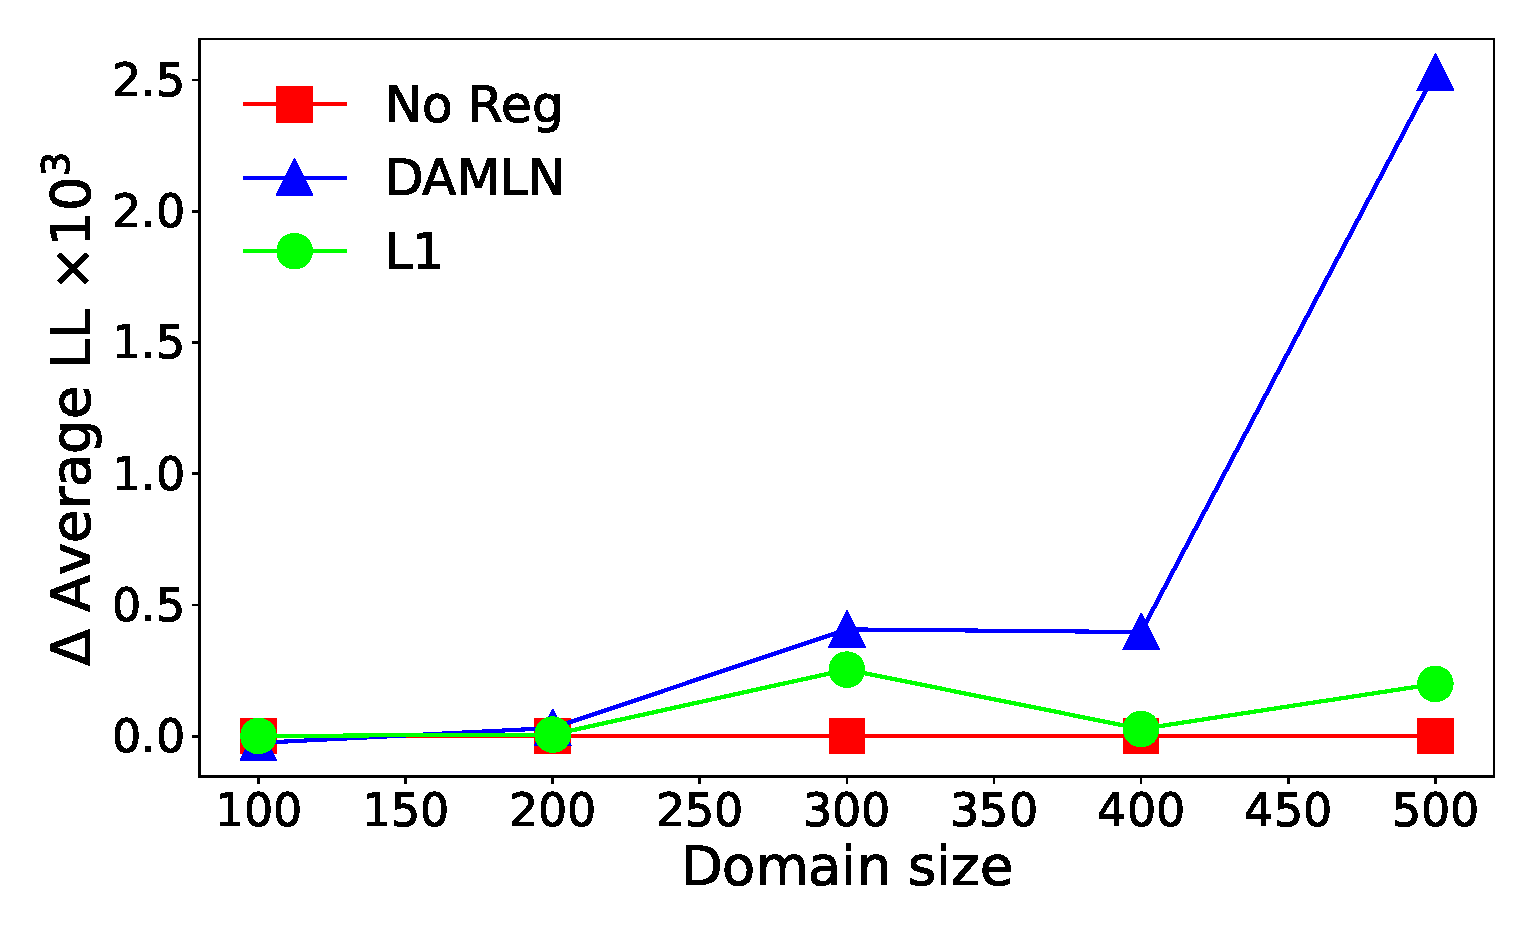
\includegraphics[width=\textwidth]{smoking_likelihoods_mean.eps}
         \caption{$\Delta$-Likelihoods (FS)}
         \label{Likelihoods (FS)}
     \end{subfigure}
     \hfill
     \begin{subfigure}[b]{0.49\textwidth}
         \centering
         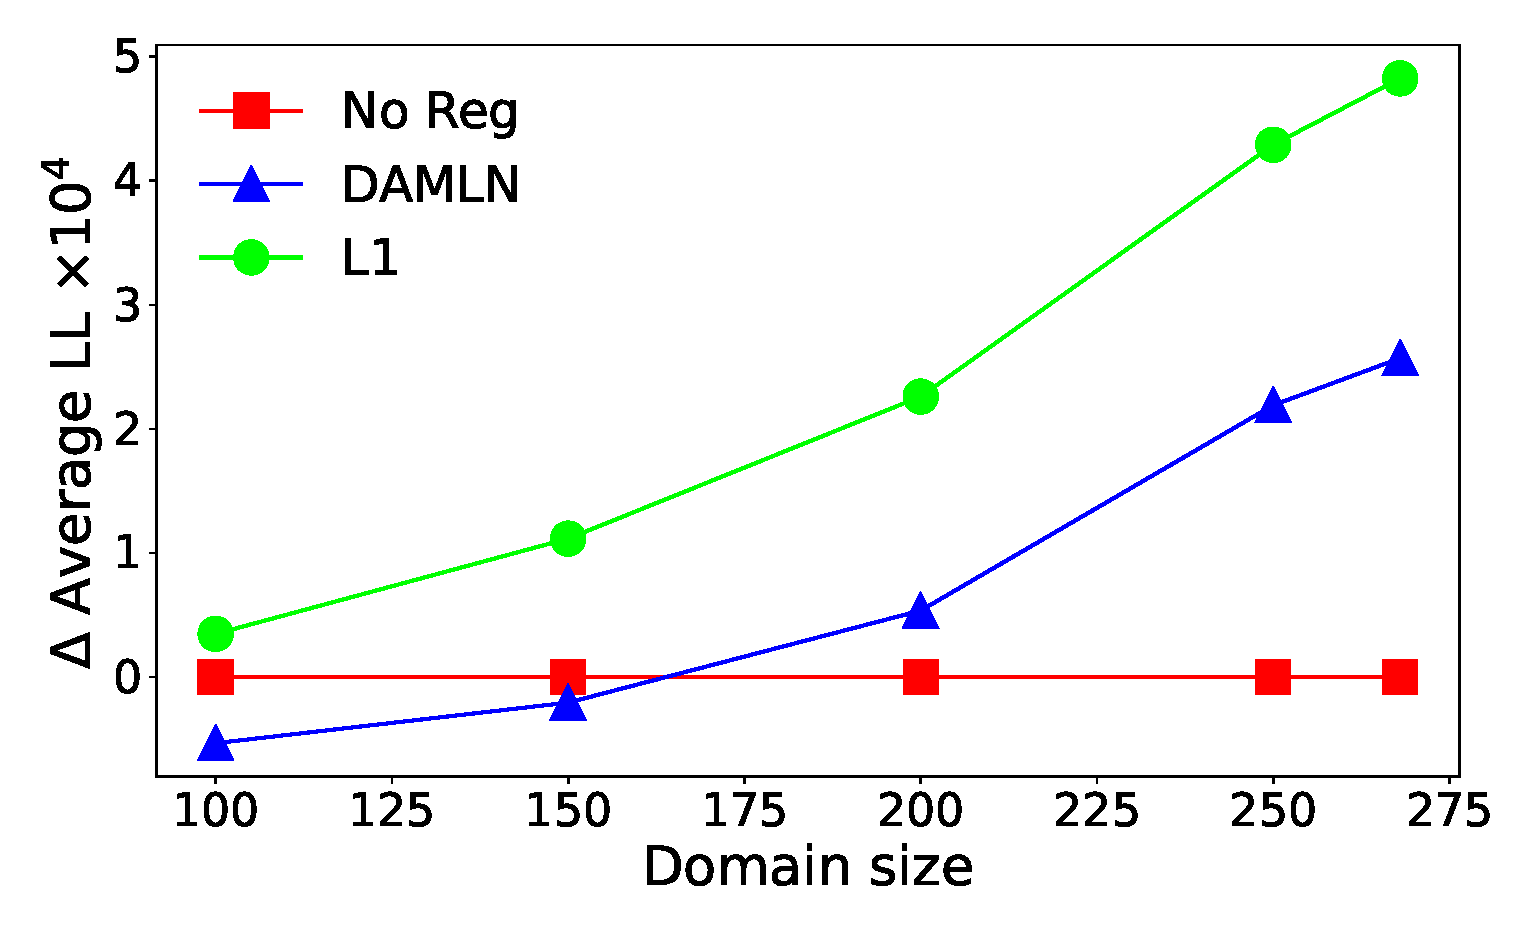
\includegraphics[width=\textwidth]{imdb_likelihoods_mean.eps}
         \caption{$\Delta$-Likelihoods (IMDB)}
         \label{Likelihoods (IMDB)}
     \end{subfigure}
     \hfill
     \begin{subfigure}[b]{0.49\textwidth}
         \centering
         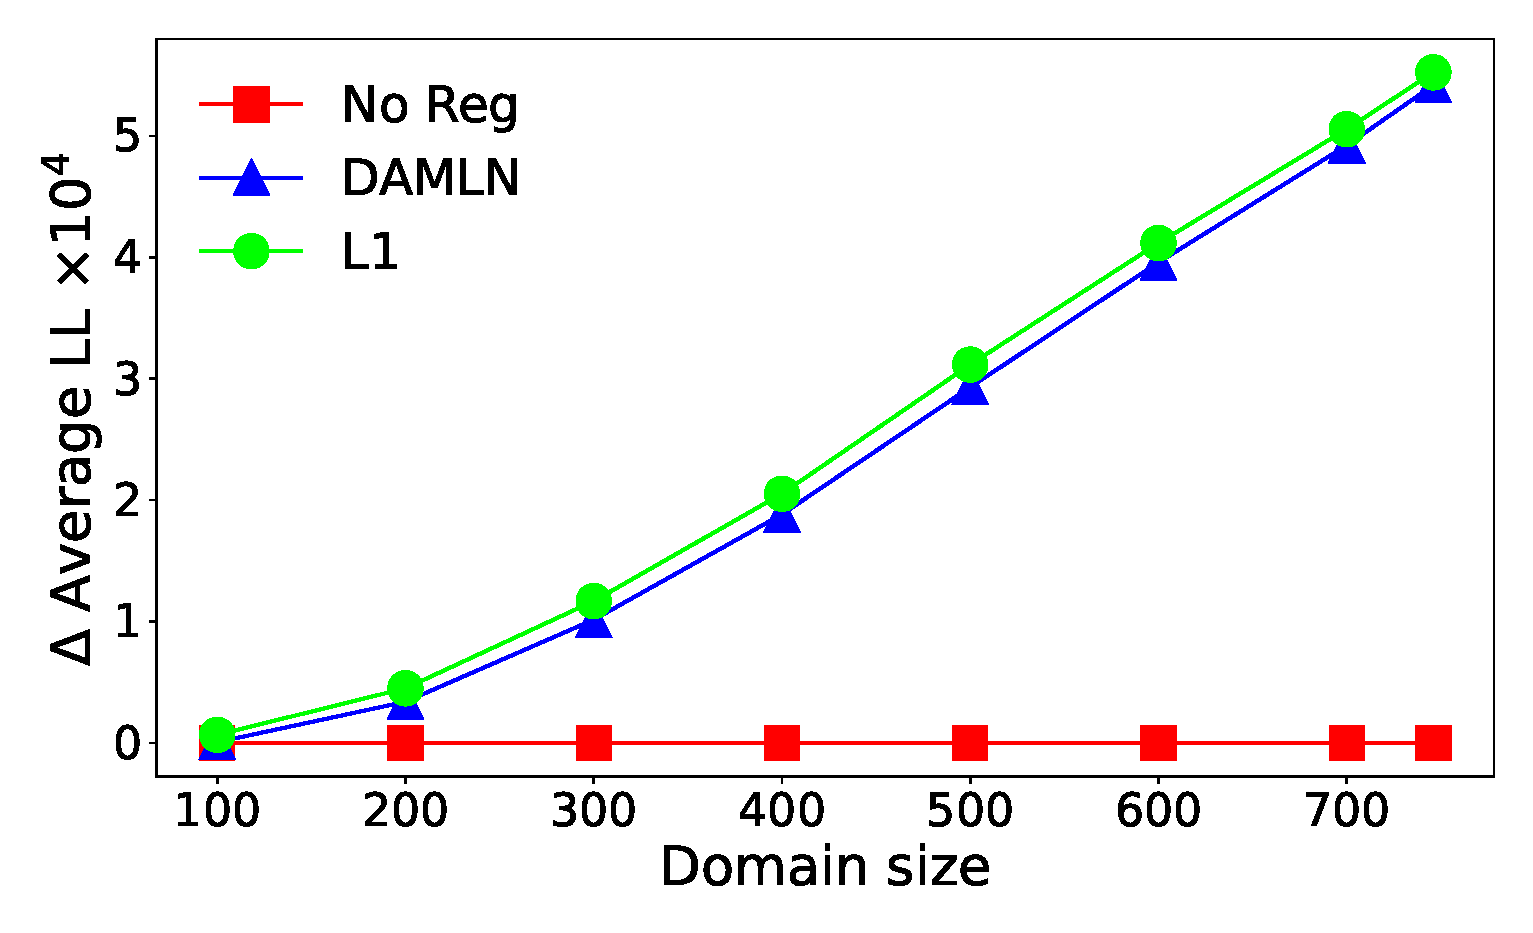
\includegraphics[width=\textwidth]{webkb_likelihoods_mean.eps}
         \caption{$\Delta$-Likelihoods (WebKB)}
         \label{Likelihoods (WebKB)}
     \end{subfigure}
     \begin{subfigure}[b]{0.49\textwidth}
         \centering
         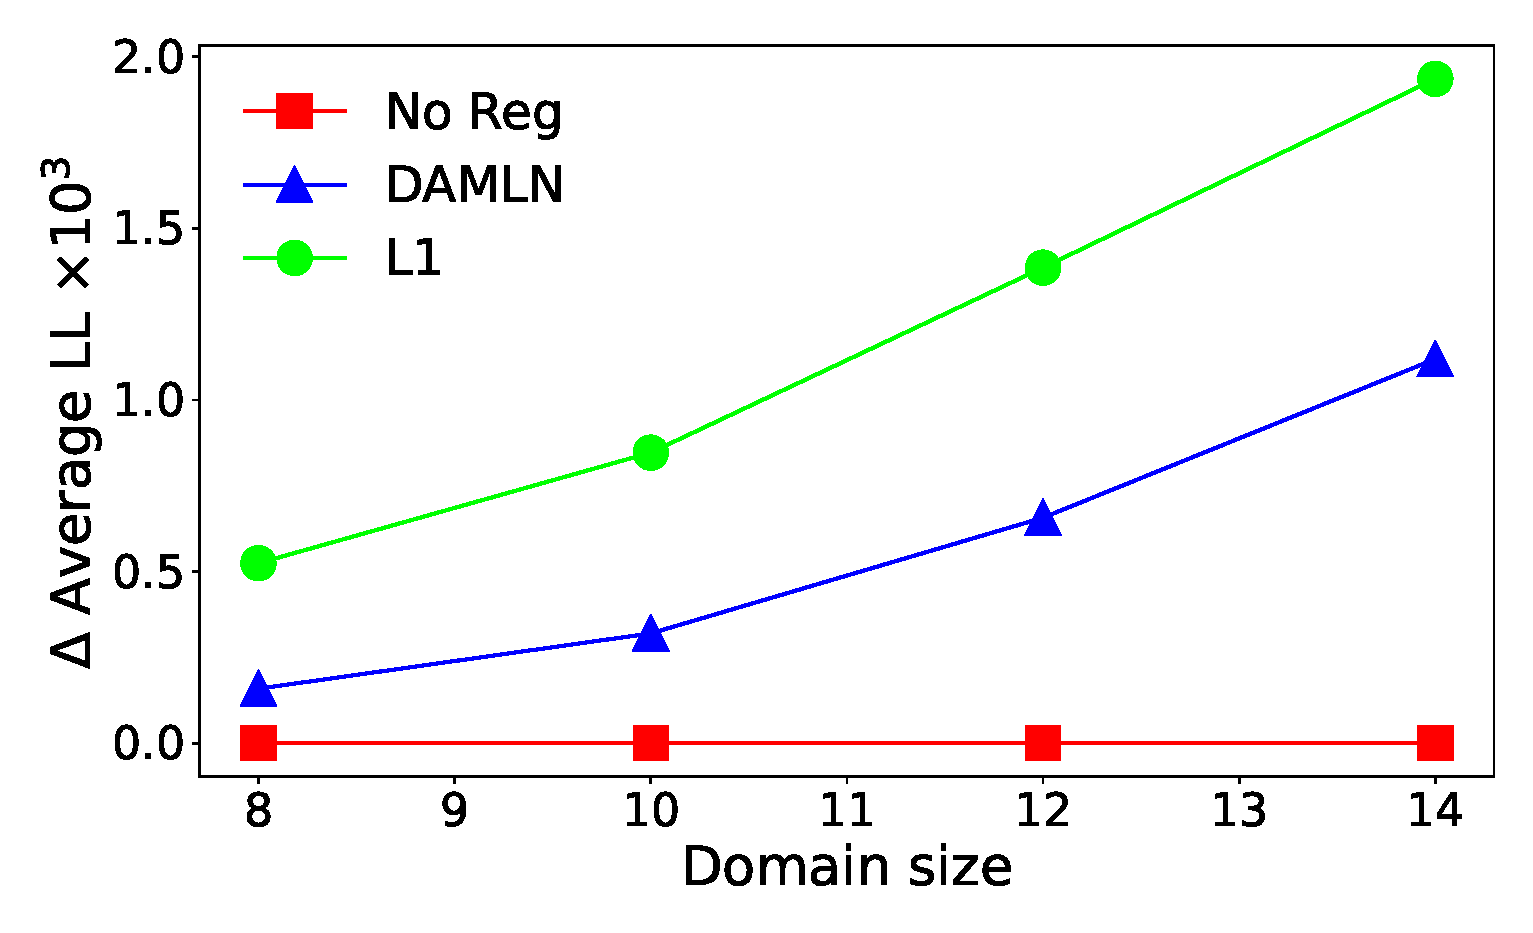
\includegraphics[width=\textwidth]{nations_likelihoods_mean.eps}
         \caption{$\Delta$-Likelihoods (Nations)}
         \label{Likelihoods (Nations)}
     \end{subfigure}
        \caption{Results for the Friends \& Smokers, IMDB, WebKB, and Nations datasets}
        \label{fig:three graphs}
\end{figure}

Discuss the phenomenon with all negative groundings which helps performance of regularization


% \input{06_rbm}
%\input{Assymptotic_Probabilities}
%\input{04_mln2rbm}
% \input{07_learning}
%\input{06_related}
% \input{08_conclusion}

%% The file named.bst is a bibliography style file for BibTeX 0.99c


% \bibliographystyle{splncs04}
\bibliographystyle{unsrt}
\bibliography{main}
% \section*{Appendix}
\subsection*{ A.1 : Lemma \ref{lem: neccesity} [Necessary]}
In this section we will make the last steps in the proof of lemma \ref{lem: neccesity} more rigorous. In the lemma we argue that, for any choice of the domain size $m$ and for any choice of $m$-worlds $(\x,\y)$ and $(\x',\y')$, we have that:
  \begin{align}
    \label{eq: lemma_2_condition}
    \sum_{i\in [u]}s_i \prod_{j\in[u]}f_{ij}^{k_{j}(\bx)} &= \sum_{i\in [u]}s_i \prod_{j\in[u]}f_{ij}^{k_{j}(\bx')} 
  \end{align}
This implies that:
\begin{equation}
    \label{eq: lem_2_conclusion}
      \forall i,j,i',j'\in [u]: f_{ij} =  f_{i'j'}  
\end{equation}
We will first infer a slightly stricter equation from \eqref{eq: lemma_2_condition}.
Since, $f_{ij} = f_{ji}$, we can see $\{f_{ij}\}$ as a symmetric $u \times u$ matrix in $\mathbb{R}_{>0}^{u\times u}$. Furthermore, $\x$ and $\x'$ can have any
1-type cardinalities $\bk = \langle k_1 ... k_u\rangle$ and $\bk'= \langle k'_1 ... k'_u\rangle$ respectively, such that $\sum_{i\in [u]}k_i = \sum_{i\in [u]}k'_i = m$. Hence, we can conclude that, for all $\bk$ and $ \bk'$ such that $\sum_{i\in [u]}k_i = \sum_{i\in [u]}k'_i$, we have that:
\begin{align}
    \label{eq: lemma_2_condition_2}
    \sum_{i\in [u]}s_i \prod_{j\in[u]}f_{ij}^{k_j} &= \sum_{i\in [u]}s_i \prod_{j\in[u]}f_{ij}^{k'_{j}} 
  \end{align}
Hence, our goal is to prove that \eqref{eq: lemma_2_condition_2} implies \eqref{eq: lem_2_conclusion}. We formally prove this statement in Lemma \ref{lemma_2}. Before proving Lemma \ref{lemma_2}, we will need to prove the following 
auxiliary lemma. 
\begin{lemma}
    \label{lemma_1}
  Let $(x_i)^{m}_{i=1}$,$(y_i)^{m}_{i=1}$ and $(a_i)^{m}_{i=1}$ be tuples of positive non-zero reals. If for all positive integers $n$: 
    \begin{equation}
      \label{eq: lemma_1}
     \sum_{i=1}^{m}a_ix_i^{n} = \sum_{i=1}^{m}a_iy_i^{n}
    \end{equation}
  then the set of entries in $(x_i)^{m}_{i=1}$ and the set of entries in $(y_i)^{m}_{i=1}$ are the same. 
  \end{lemma}
  % \begin{proof}
  %   Let us assume to the contrary that $\sum_{i=1}^{m}x_i > \sum_{i=1}^{m}y_i$. Let $x_{l}$ and $y_{l'}$ be the maximal elements in $\{x_i\}^{m}_{i=1}$ and $\{y_i\}^{m}_{i=1}$ respectivaly.
  %   Since,  $\sum_{i=1}^{m}x_i > \sum_{i=1}^{m}y_i$, we have that $x_{l} > y_{l'}$. 
    
  %   But as $n$ tends to infinity, due to \eqref{eq: lemma_1}, we must have that $a_lx_l^{n} = a_{l'}y_{l'}^{n} $, which is true only if $x_l = y_{l'}$, which contradicts our assumption that $$
  % \end{proof}
  \begin{proof}Let $\{u_{i}\}^{p}_{i=1}$ and  $\{v_{i}\}^{q}_{i=1}$ be the set of unique entries in $(x_i)^{m}_{i=1}$ and $(y_i)^{m}_{i=1}$ respectively. Also, without loss of generality, we may assume an ordering such that $u_1 > u_2> ... >u_{p} $ and $v_1 > v_2> ...>v_{q} $ and also that $q\geq p $. We can rewrite \eqref{eq: lemma_1} as:
  \begin{equation}
    \label{eq: lemma_1_equivalence}
   \forall n \in \mathbb{Z^{+}}:  \sum_{i=1}^{p}c_iu_i^{n} = \sum_{i=1}^{q}d_iv_i^{n} 
  \end{equation}
  As $n$ grows the leading term on LHS is $c_1u_{1}^{n}$ and on the RHS is $d_1v_{1}^{n}$. Hence, it must be :
  
  \begin{equation*}
    \forall n \in \mathbb{Z^{+}}: c_1 u_{1}^{n}  = d_1 v_{1}^{n} 
  \end{equation*}
  Since, $u_1,v_1,c_1$ and $d_1$ are non-zero positive reals, we can conclude that $u_1=v_1$ and $c_1 = d_1$. Hence, we may subtract $c_1 u_{1}^{n}$ from both sides in \eqref{eq: lemma_1_equivalence} to get :
  \begin{equation}
    \label{eq: lemma_1_equivalence_1}
   \forall n \in \mathbb{Z^{+}}:  \sum_{i=2}^{m'}c_iu_i^{n} = \sum_{i=2}^{m''}d_iv_i^{n} 
  \end{equation}
  We may now repeat the aforementioned argument and infer that $u_2=v_2$ and $c_2 = d_2$. Furthermore, repeating this argument $p$ times, we can infer that $\{u_i\}^{p}_{i=1} = \{v_i\}^{p}_{i=1}$, leaving us with $0 =\sum_{i=q-p+1}^{p}d_iv_i^{n}$, which is a contradiction, hence, $p=q$. Hence, we have that $\{u_{i}\}^{p}_{i=1}$ = $\{v_{i}\}^{q}_{i=1}$. Hence, completing the proof.
  \end{proof}
  
  
  \begin{lemma}
    \label{lemma_2}
  Let $F = (f_{ij}) \in \mathbb{R}_{>0}^{u \times u}$ be a symmetric matrix and let $(s_i)^{u}_{i=1} \in \mathbb{R}_{>0}^{u}$. If for all $\bm{k} = \langle k_1,...,k_u \rangle$ and $\bm{k'} = \langle k'_1,...,k'_u \rangle $ such that $k_i,k'_i \in \mathbb{Z^{+}}$ and $\sum_{i=1}^{u}k_i = \sum_{i=1}^{u}k'_i$, we have that: 
    \begin{equation}
      \label{eq: lemma_2}
  \sum_{i=1}^{u}s_i\prod_{j\in [u]}f_{ij}^{k_{j}} = \sum_{i=1}^{u}s_i\prod_{j\in [u]}f_{ij}^{k'_{j}}
    \end{equation}
  then 
  \begin{equation*}
    \forall i,j,i',j' : f_{ij} = f_{i'j'}
  \end{equation*}
  \end{lemma}
  
  \begin{proof}
  Let $\bm{k}$ be such that $k_p=n$, let $k_i = 0$ for all $i \neq p$. Let $\bm{k'}$ be such  that $k_q=n$ and $k_i = 0$ for all $i \neq q$. Then due to \eqref{eq: lemma_2}, we have that:
  
  \begin{equation}
  \forall n \in \mathbb{Z^{+}}: \sum_{i=1}^{u}s_i(f_{ip})^{n} = \sum_{i=1}^{u}s_i(f_{iq})^{n}
  \end{equation} 
  Hence, due to Lemma \ref{lemma_1}, we have that the entries in $(f_{ip})^{u}_{i=1}$ and $(f_{iq})^{u}_{i=1}$ form the same set. A similar argument can 
  be repeated for any pair of columns. Hence, all columns in $F$ have the same set of entries, we denote the set of such entries as $U$. 
  
  Now, let $n = uk$ where $k \in \mathbb{Z}^{+}$, and $\bm{k}$ such that $k_i=k$ for all $i \in [u]$ and $\bm{k'}$ such that $k'_q=n$ and $k'_i = 0$ for all $i \neq q$. Then due to \eqref{eq: lemma_2}, we have that:
  \begin{align*}
    \forall k \in \mathbb{Z^{+}}: \sum_{i=1}^{u} s_i \prod_{p\in[u]}f_{ip}^{k} &= \sum_{i=1}^{u}s_i(f_{iq})^{uk}\\
    \forall k \in \mathbb{Z^{+}}: \sum_{i=1}^{u} s_i \bigl(\prod_{p\in[u]}f_{ip}\bigr)^{k} &= \sum_{i=1}^{u}s_i (f_{iq}^{u}\bigr)^{k}
  \end{align*} 
  As $k$ grows the leading term on left hand side and right hand side must agree for the equality to hold. Let $c_{i'} \bigl(\prod_{p\in[u]}f_{i'p}\bigr)^{k}$ and $d_{i''} (f_{i''q}^{u}\bigr)^{k}$ be the leading terms on RHS and LHS respectively.
  Hence,
  \begin{equation}
    \label{eq: compare_uni_edge}
    \forall k \in \mathbb{Z^{+}} : c_{i'} \bigl(\prod_{p\in[u]}f_{i'p}\bigr)^{k} = d_{i''} (f_{i''q}^{u}\bigr)^{k} 
  \end{equation}
  which implies that $\prod_{p\in[u]}f_{i'p} = f_{i''q}^{u}$. Now, clearly $f_{i''q}$ is equal to the maximum term in $U$ say $s$. Now, $\prod_{p\in[u]}f_{i'p}$ is a product of all  the terms in 
  the $p^{th}$ matrix column of $F$. Hence, $\prod_{p\in[u]}f_{i'p} \leq s^{u}$. Hence, due to \eqref{eq: compare_uni_edge}, we have that:
  
  \begin{equation*}
    \forall i,j,i',j' : f_{ij} = f_{i'j'}
  \end{equation*} 
  \end{proof}
  
  
  
 
\end{document}
